\chapter{Introduction to tRNA biology}
\label{chap4}


This chapter is related to the paper: "[insert title here]" [insert reference here].
This paper describes a method for quantifying tRNA aminoacylation levels by making several improvements and combining the best of previous tRNA-seq methods.
The method is then tested using realistic sample conditions and an improved data processing strategy is described and tested.
All the essential findings of this chapter are described in the publication, and thus this should be preferred for most practical applications.
However, the publication focuses on the elements of method development that work and largely omits observations from experiments that failed.
I shall here correct this bias towards successful experiments, add new observations and interpretations, expand the background and discuss the many trade offs and pitfalls.


\section{Background}
Basic background like:
Purpose (protein synthesis).
Transfer RNA (tRNA).
Abundance compared to total RNA.
Length and sequencing similarity.
Transcripts of the same codon and copy number.

Transcription, intron splicing and CCA addition.
Modifications and their purpose (wobble, decoding etc.).
Modifications in tubeculosis \cite{Tomasi2023-wg}

Compartmentalization (cyto, mito, chloroplasts)

Secondary structure.
Discriminator base.

Aminoacylation, enzyme specificity and ester bond stability.



\begin{figure}
     \centering
     \begin{subfigure}[b]{0.4\textwidth}
         \centering
         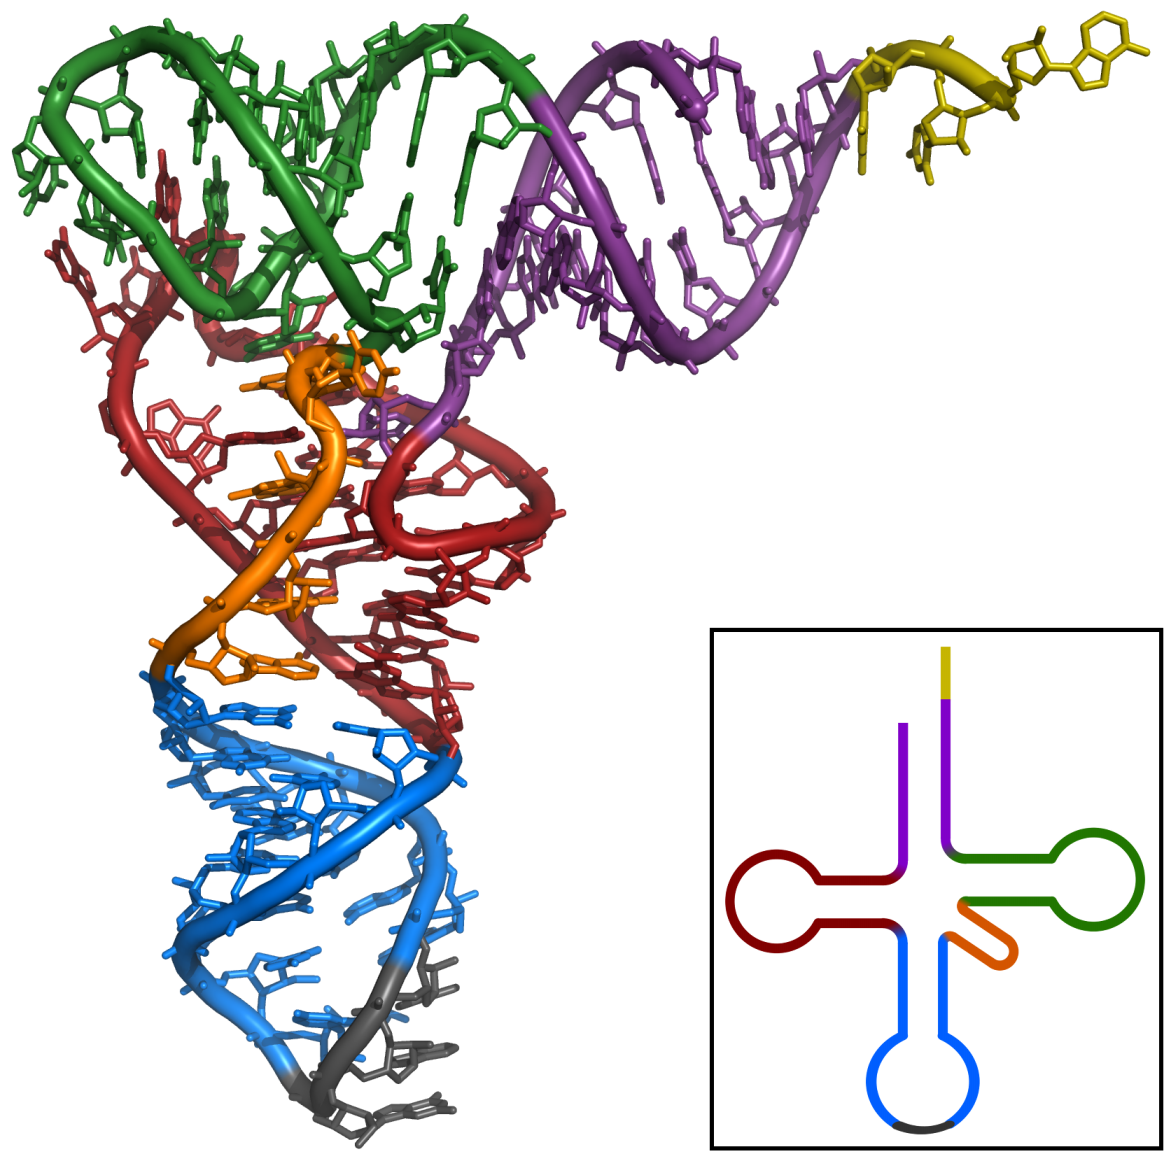
\includegraphics[width=\textwidth]{figures/chap4/TRNA-Phe_yeast_1ehz.png}
         \caption{}
         \label{fig:tRNA_3d_struct}
     \end{subfigure}
     \hfill
     \begin{subfigure}[b]{0.3\textwidth}
         \centering
         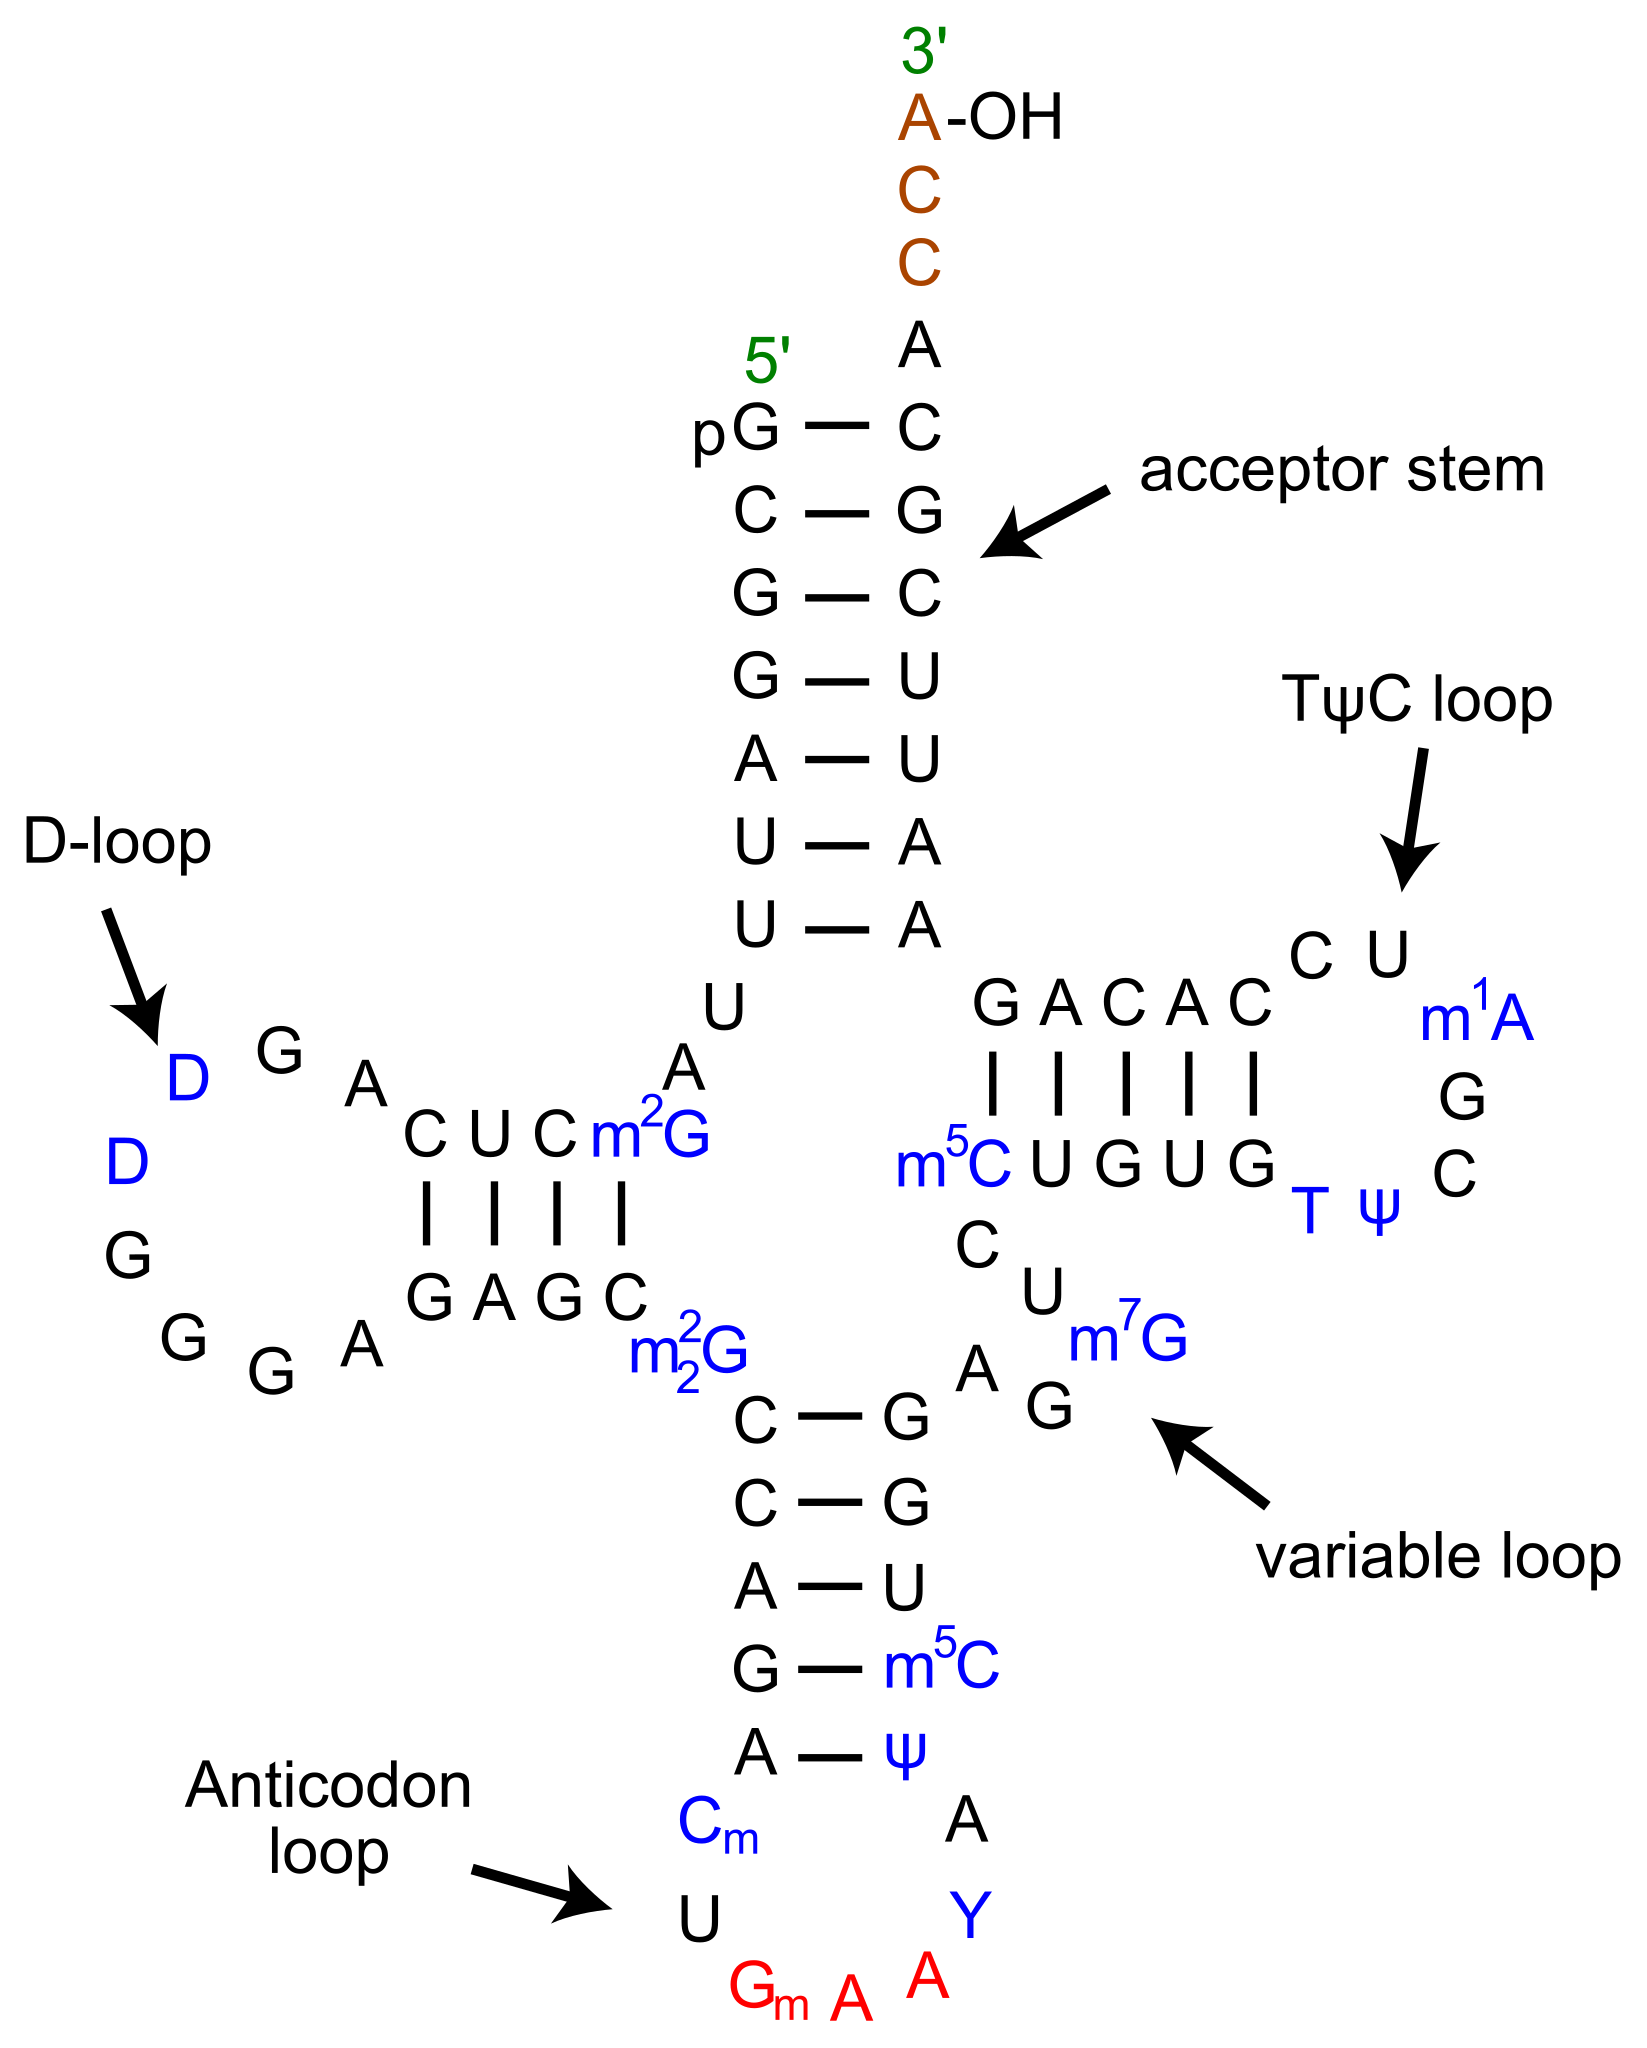
\includegraphics[width=\textwidth]{figures/chap4/TRNA-Phe_yeast_en.png}
         \caption{}
         \label{fig:tRNA_2d_struct}
     \end{subfigure}
     \hfill
     \begin{subfigure}[b]{0.2\textwidth}
         \centering
         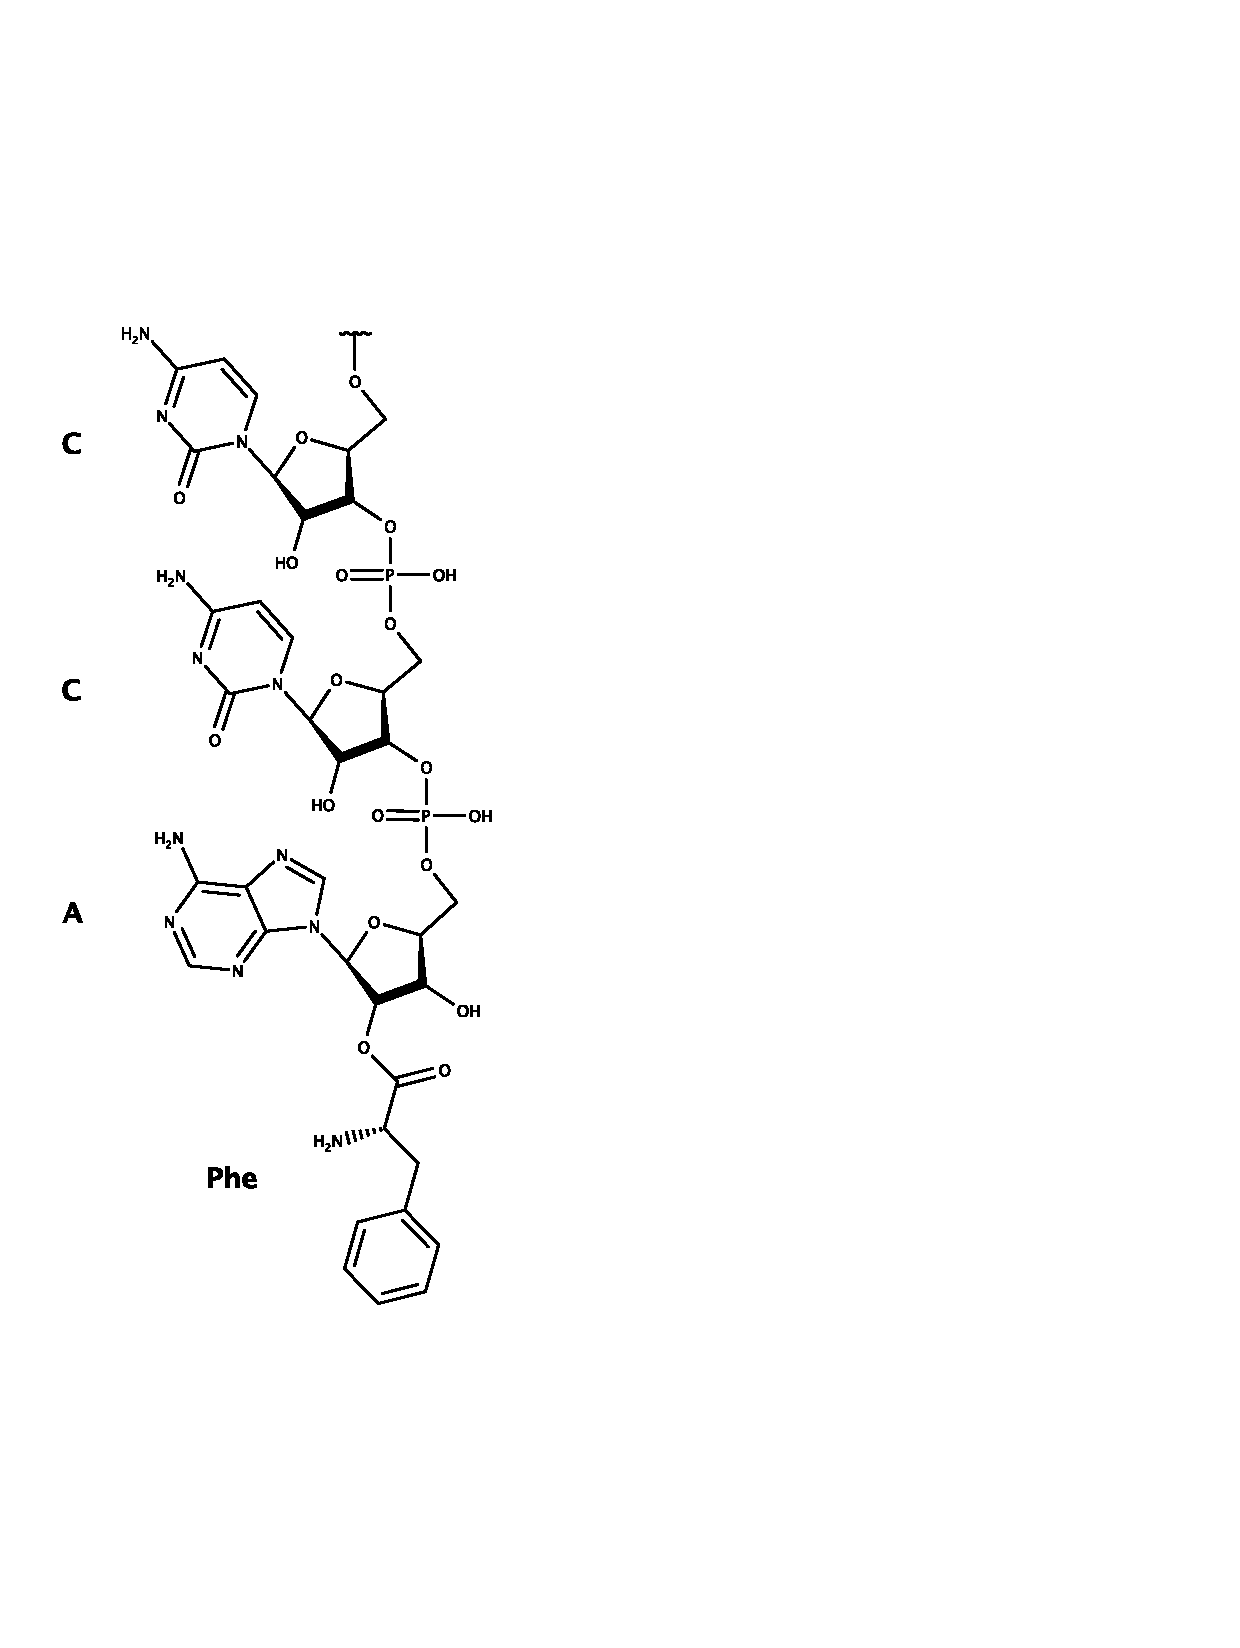
\includegraphics[width=\textwidth]{figures/chap4/CCA_Phe.pdf}
         \caption{}
         \label{fig:tRNA_CCAester}
     \end{subfigure}
        \caption[tRNA structural overview]{
        (a) Three dimensional structure of a tRNA colored by secondary structure elements shown in the insert, (b) secondary structure of a tRNA with names of the structural elements and some common base modifications, (c) the 3' CCA of a tRNA aminoacylated with phenylalanine.
        (a) and (b) from Yikrazuul, \href{https://creativecommons.org/licenses/by-sa/3.0}{CC BY-SA 3.0}, via Wikimedia Commons.
        }
\end{figure}





\begin{figure}
    \centering
    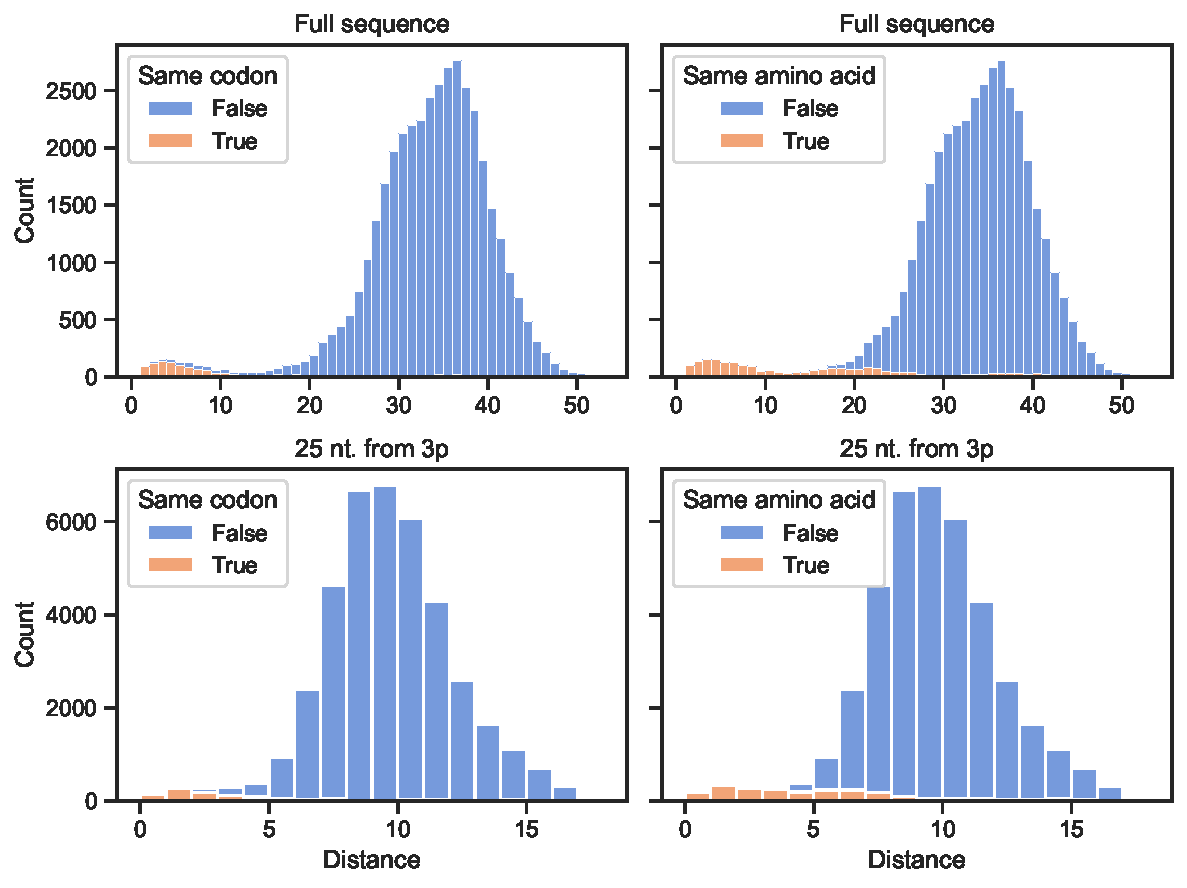
\includegraphics[width=0.98\textwidth]{figures/chap4/tRNA_dist_hist.pdf}
    \caption[Pairwise tRNA distance histogram]{Histogram of the distances between tRNA transcripts after pairwise Needleman–Wunsch alignment.
    Distance is counted as the number of mismatches and gaps.
    The top row shows full sequence transcripts, the bottom row shows the last 25 nt. of each transcript.
    Distances are broken down by being between transcripts of the same codon or not, and same amino acid or not. Source: krdav Github \href{https://github.com/krdav/thesis_plotting/blob/main/tRNA_stats/plot_data.ipynb}{thesis\_plotting/tRNA\_stats}}
    \label{fig:dist_hist}
\end{figure}




\begin{table}[!htb]
\begin{tabular}{|l|p{0.85\textwidth}|}
\hline
Length & tRNAs \\ \hline
62     & m\=/Ser\=/AGC \\ \hline
68     & m\=/Arg\=/CGA \\ \hline
69     & m\=/Cys\=/UGC, m\=/Thr\=/ACA, m\=/Tyr\=/UAC \\ \hline
71     & m\=/Met\=/AUG, m\=/Trp\=/UGA, m\=/Pro\=/CCA, m\=/Gly\=/GGA, m\=/Asp\=/GAC \\ \hline
72     & m\=/Ser\=/UCA, m\=/Val\=/GUA, m\=/His\=/CAC, m\=/Ile\=/AUC, m\=/Glu\=/GAA, m\=/Ala\=/GCA \\ \hline
73     & c\=/Cys\=/UGC, m\=/Lys\=/AAA \\ \hline
74     & m\=/Phe\=/UUC, c\=/Gly\=/GGC, m\=/Leu\=/CUA, c\=/Ala\=/GCA, c\=/Gly\=/GGG \\ \hline
75     & c\=/Gln\=/CAG, c\=/Tyr\=/UAC, c\=/Ala\=/GCG, c\=/Ala\=/GCA, c\=/Gly\=/GGA, c\=/Pro\=/CCA,   c\=/Gln\=/CAA, c\=/Glu\=/GAG, c\=/Pro\=/CCU, c\=/Thr\=/ACA, c\=/Val\=/GUU, m\=/Gln\=/CAA, c\=/Asp\=/GAC,   c\=/Ala\=/GCU, c\=/Pro\=/CCG, c\=/Thr\=/ACG, c\=/His\=/CAC, c\=/Glu\=/GAA, c\=/Cys\=/UGC, c\=/Trp\=/UGG,   c\=/iMet\=/AUG \\ \hline
76     & c\=/Val\=/GUA, c\=/Arg\=/AGG, c\=/Tyr\=/UAU, c\=/Val\=/GUG, c\=/Ala\=/GCU, c\=/Tyr\=/UAC,   c\=/Arg\=/CGG, c\=/Met\=/AUG, m\=/Asn\=/AAC, c\=/Cys\=/UGC, c\=/Lys\=/AAG, c\=/Val\=/GUU, c\=/Arg\=/CGU,   c\=/Arg\=/CGA, c\=/Lys\=/AAA, c\=/Thr\=/ACA, c\=/Arg\=/AGA, c\=/Phe\=/UUC \\ \hline
77     & c\=/Thr\=/ACU, c\=/Ile\=/AUU, c\=/Ile\=/AUC, c\=/Lys\=/AAG, c\=/Asn\=/AAC, c\=/Leu\=/UUG,   c\=/Thr\=/ACA, c\=/Thr\=/ACG, c\=/Arg\=/AGA, c\=/Phe\=/UUC, c\=/Ile\=/AUA \\ \hline
78     & m\=/Leu\=/UUA, c\=/Asn\=/AAC \\ \hline
85     & c\=/Ser\=/UCG, c\=/Leu\=/CUU, c\=/Ser\=/AGC, c\=/Ser\=/UCU, c\=/Leu\=/CUA, c\=/Ser\=/UCA \\ \hline
86     & c\=/Leu\=/UUA, c\=/Leu\=/UUG, c\=/Leu\=/CUG \\ \hline
87     & c\=/Ser\=/AGC, c\=/Leu\=/UUG \\ \hline
90     & c\=/SeC\=/UGA \\ \hline
\end{tabular}
\caption[Length distribution of tRNAs]{Mature human tRNA transcript lengths and the distribution among amino acids and codons. The tRNA column is populated with entries formatted as [cyto/mito]-[amino acid]-[codon] with [cyto/mito] indicated by c/m, [amino acid] indicated by the three letter amino acid code. Source: krdav Github \href{https://github.com/krdav/thesis_plotting/blob/main/tRNA_stats/plot_data.ipynb}{thesis\_plotting/tRNA\_stats}}
\end{table}
















\section{Quantifying aminoacylation}

Quantification of \textit{in vivo} transfer RNA (tRNA) aminoacylation is complicated by the many, highly similar, tRNA transcripts.
It was first with Northern blotting that tRNA transcripts could be resolved with sufficient resolution.
Aminoacylation can then be resolved by differential migration during electrophoresis and following probe quantification the level of aminoacylation, or charge, can be calculated \cite{Ho1987-ug, Varshney1991-zp, Stenum2017-wn}.





Multiple methods for quantifying aminoacylation these are...


\subsection{Northern blotting}
qwerty

\subsection{tRNA-seq}
Overview of the tRNA-seq methods.
Overview of the periodate-cleavage reaction.
Briefly, mention the array based tech introduced right before RNAseq.
Transition into giving an overview of each major advance in the methods.

\subsubsection{Zheng 2015}
Tao Pan RNAseq.
Extended by Evans 2017 to measure aminoacylation
\cite{Zheng2015-kj}


\subsubsection{Shigematsu 2017}
YAMAT seq


\subsubsection{Behrens 2021}
ghjm

\subsubsection{Others}
Here described other minor methodological advances/differences.
E.g. Wang [specifically amplified by GGT-ending primer during]







\subsection{The Malaprade-elimination reaction}
Dig deep into this reaction, the previous use, the chemistry etc.
This facilitates the discrimination between aminoacylated and unaminoacylated tRNA.
First used in Evans 2017, heavily inspired by the previous array based paper from Tao Pan's group.


\subsection{A lack of quantification rigor}
qwerty




\section{Strategy to improve tRNA-seq based aminoacylation quantification}


\section{Data processing}

\subsection{The alignment problem}
Blob on alignment:

* Maybe turn this into a wider discussion of annotation strategies and why it might be optimal to use masked sequences because this applies the least number of assumptions. A positional gap penalty would also help in that regard. HMM would be very strong but also would also make some assumptions about the modified sites that could be problematic in different contexts e.g. the HMM is fitted on data with a particular position always is modified but then in a biological context this modification is lost.
* Advantages: formalized model that calculated probabilities, can model site interactions, can model gaps and RT stops.
Modeling RT stops could be problematic though since it could easily vary depending on RT conditions, polymerases etc.
* Disadvantage: very slow, probably has to be refitted for new datasets because of slightly different RT conditions, also has to be refitted to take into account any biological changes in modification penetrance
* Pick a subset of reads with long alignments where the top scoring reference is several score points away from the runner up.
* Use these sequences to make an HMM for each annotation
* Run the HMMs on all sequences and calculate the annotation probability without the RT fall-off.
* Select all the sequences with an annotation with high HMM probability * away from the second best annotation.
* Refit the HMMs on these sequences.
* Run the HMMs on all sequences and calculate the annotation probability, this time with the RT fall-off included.
* Select sequences and refit HMM.
* Perform enough iterations to converge.





\section{Results}


\section{Methods}

\section{Discussion}



